% !TEX root = tesis.tex

\chapter{Evaluating Performance of Bayesian Prediction Algorithm}
\label{sec:results}

In this chapter, we test the \emph{Prediction Algorithm} presented in \cref{sec:inference_methodology} with the data present on the graph.

\section{Experimental Environment}
\label{subsec:experimental_environment}

All the tests are being performed in a single \texttt{Linux 3.16} server with 16 \texttt{Intel Xeon D-1540} cores with 2GHz of power, and 128GByte of RAM\@.

The programming environment consists of \texttt{Python 2.7.9}, which along with the libraries \texttt{numpy 1.12.1}, \texttt{scipy 0.18.1}, \texttt{pandas 0.19.2}, and \texttt{scikit-learn 0.18}\cite{scikit-learn} were used for creating both the \emph{Bayesian Algorithm}, all the \emph{Machine Learning} methods described in \cref{sec:comparison}, and the many programs created for feature engineering.

The experimentation was achieved using the previous libraries, using the amazing \texttt{Jupyter 5.1.0} notebooks as an environment and \texttt{matplotlib 1.5.2} and \texttt{seaborn 0.7.1} to create the graphs used in this thesis.

\section{Data Partitioning}
\label{sec:data_partitioning}

\subsection{Train Test Split}
\label{subsec:train_test_split}

As with many other classification problems, the \emph{Bayesian Algorithm} is prone to overfitting~\cite{mitchellml1997}.
In this particular case, since the information presented in \cref{subsec:income_homophily} shows that users tend to communicated with users of the same socioeconomic level, by running the algorithm in the complete data and using the same users as part of the features and of the labels, we would erroneously be having more data per user than we would have when modelling the problem.

Since the input data used in this experiment comes from $B$, the banking information of the users in the telco, we can avoid most of the effects of overfitting separating the data into a \emph{Training Set} and a \emph{Testing Set}, where the data in $B$ is separated into two disjoint groups as shown in \cref{eq:train_test_split}.

\begin{equation}
\label{eq:train_test_split}
	\begin{gathered}
		\begin{aligned}
			B_{\train} &\subseteq B & \left| B_{\train} \right| = 0.8 &\cdot \left| B \right| \\
			B_{\test} &\subseteq B & \left| B_{\test} \right| = 0.2 &\cdot \left| B \right|
		\end{aligned} \\
		B_{\train} \cap B_{\test} = \varnothing
	\end{gathered}
\end{equation}

\subsection{Erasing Uninformative Data}
\label{subsec:erasing_uninformative_data}

The \emph{Social Graph} $G = \left< V, E \right>$, which contains information about the communication networks of the users in this dataset is extremely sparse.
Because of the property and that $\left| B \right| \ll \left| V \right|$, the vast majority of users don't have any kind of contact with users of the bank.
For this reason it is useless to evaluate the performance of the algorithm using all the nodes, and therefore the \emph{Testing Set} used in this thesis will instead focus on the bank users that have at least one contact with another bank user.
This approach is formalized in \cref{eq:inner_graph}.

\begin{equation}
\label{eq:inner_graph}
\begin{gathered}
\hat{E} = \left\{ e \in E \mid e_o \in B_{\train} \lor e_d \in B_{\train} \right\} \\
\hat{B}_{\test} = B_{\test} \cap \left( \hat{E}_o \cup \hat{E}_d \right)
\end{gathered}
\end{equation}

The accuracy of this approach depends of the value of $\varpi$, which is one of $\calls$, $\etime$, $\sms$, or $\contacts$ and defines which property of the users that's used as a feature for the classification.
If $\varpi = \contacts$, then this approach works perfectly.
However, it is possible that for other values of $\varpi$ there won't be any information available in $\hat{B}_{\test}$ in the case of users who either didn't receive any call from a bank user or didn't receive any message.

\Cref{eq:inner_graph_call,eq:inner_graph_sms} formalize new variables to use for informative data in those cases.

\begin{equation}
\label{eq:inner_graph_call}
\begin{gathered}
\hat{E}^{\calls} = \left\{ e \in E \mid e_c > 0 \land \left( e_o \in B_{\train} \lor e_d \in B_{\train} \right) \right\} \\
\hat{B}^{\calls}_{\test} = B_{\test} \cap \left( \hat{E}^{\calls}_o \cup \hat{E}^{\calls}_d \right) \\
\end{gathered}
\end{equation}

\begin{equation}
\label{eq:inner_graph_sms}
\begin{gathered}
\hat{E}^{\sms} = \left\{ e \in E \mid e_s > 0 \land \left( e_o \in B_{\train} \lor e_d \in B_{\train} \right) \right\} \\
\hat{B}^{\sms}_{\test} = B_{\test} \cap \left( \hat{E}^{\sms}_o \cup \hat{E}^{\sms}_d \right)
\end{gathered}
\end{equation}

\subsection{Rebalancing Labels}
\label{subsec:rebalancing_labels}

Since the testing data $B_{\test}$ was a random subsample of a balanced set (see \cref{subsec:train_test_split,subsec:discrimination_by_wealth}), it was also balanced itself. However, since \emph{High Income} users tend to communicate more often than \emph{Low Income} ones, $\hat{B}_{\test}$ is unbalanced and has a significant bias for high-income users.

Since the income categories tend to be balanced in the real world, this isn't wanted. However, since it is not necessary to use the entire \emph{Testing Set} for testing the algorithm, a simple way would be to create a new, balanced, and final testing set, $\Upsilon \subseteq \hat{B}_{\test}$ containing all users from $\hat{B}_{\test}$ \emph{Low Income}, along with a random sample of the same size with \emph{High Income}.

\begin{equation}
\label{eq:upsilon}
\begin{gathered}
\begin{aligned}
\Upsilon^{\low} &= \hat{B}_{\test} \cap H_1 \\
\Upsilon^{\high} &\subseteq \hat{B}_{\test} \cap H_2
\end{aligned} \\
\left| \Upsilon^{\low} \right| = \left| \Upsilon^{\high} \right| \\
\Upsilon = \Upsilon^{\low} \cup \Upsilon^{\high}
\end{gathered}
\end{equation}

$\Upsilon$ will be the only \emph{Testing Set} used from now on, while $B_{\train}$ will be used as training set.

Additionally, the sets $\Upsilon^{\calls}$ and $\Upsilon^{\sms}$ refer to similar sets which are taken from users from the \emph{Testing Set} that had at least one call or sent at least one SMS, respectively, to another user in the \emph{Training Set}.

\subsection{The Inner and Outer Graph}
\label{subsec:inner_outer_graph}

Most of the rest of the thesis will use the subgraphs $\Upsilon$, later called the \emph{Inner Graph}, containing only users with at least one labeled neighbour, and $B_{\test}$, the \emph{Outer Graph}, containing all users.
For simplicity sake, from now on the \emph{Outer Graph} $B_{\test}$ will be referred to as $\Omega$, and the unbalanced outer graph (which is not used after this section) as $\hat{\Omega}$.

As shown in \cref{subsec:rebalancing_labels}, the labels have roughly the same amount of high income and low income users.

The \emph{Outer Graph} $\Omega$ is not used in this section, as the \emph{Bayesian Algorithm} requires some information about the \emph{Socioeconomic Level} of the neighbours of the users used in the prediction. However, it is used as one of the main inputs for generating features in the later \cref{sec:comparison}.

\subsection{Set Magnitudes}

While the new set $\Upsilon$ contains significantly less users than the original set $B$, it still has a sufficient amount of people to make a prediction. \Cref{tab:partition_numbers} shows the number of users that remain after every trim used in this Subsection, along with the ratio of users which we would be able to assign an \emph{Income Category} using these datasets assuming the real data is equally distributed from the \emph{Test Data}.

\begin{table}
\centering
\begin{tabular}{l r r r c}
\toprule
Set & Total Size & High Income & Low Income & Ratio \\
\midrule
$B$ & \num{5402959} & \num{2702628} & \num{2700331} & \NA{} \\
$\Omega$ & \num{1080592} & \num{540526} & \num{540066} & \NA{} \\
$\hat{\Omega}$ & \num{53691} & \num{35215} & \num{18476} & \num{1.000} \\
$\Upsilon$ & \num{36952} & \num{18476} & \num{18476} & 1.000 \\
$\Upsilon^{\calls}$ & \num{30715} & \num{15653} & \num{15062} & 0.831 \\
$\Upsilon^{\sms}$ & \num{11909} & \num{6046} & \num{5863} & 0.322 \\
\bottomrule
\end{tabular}
\caption{Amount of users in the \emph{Testing Set} after trimming it several times to prevent overfitting while keeping the labels balanced}
\label{tab:partition_numbers}
\end{table}

\section{Optimizing $\Theta$}
\label{subsec:optimize_theta}

In \cref{subsec:modelling_users} we define the variable $\Theta$, which is defined as the quantile used to define the \emph{Posterior Probability} $p_v$ of a user $v$ being part of the higher income category.
Choosing a good value of $\Theta$ is an essential step in creating a correct algorithm since it is the most important constant of \cref{eq:beta_theta_ppf}, one of the crucial parts for finding the category of an user.

As explained in \cref{subsec:modelling_users}, it is convenient to use \emph{Jeffrey's Prior} as the prior distribution for this variable.
However, knowing how it will affect the prediction of the category of each $v$ for every $\varpi \in \left\{ \calls, \etime, \sms, \contacts \right\}$ will allow us to get a good posterior value.

The main hypotheses tested in this part of the theses were two assumptions.

\begin{enumerate}
	\item The optimal value of $\Theta$ will be the same for any $\varpi$.
	\item Overlooking extreme values, the value of $\Theta$ won't improve or deteriorate the prediction.
\end{enumerate}

As \cref{tab:besttheta,fig:theta} show, both hypotheses are false.

\begin{figure}
\centering
\includegraphicsmaybe{figures/theta.png}
\caption{The \emph{Area Under the Curve} for different $\Theta$ and every possible $\varpi$. This is the preliminary version of the analysis seen in \cref{subsec:algorithm_performance}}.
\label{fig:theta}
\end{figure}

\begin{table}
\centering
\begin{tabular}{>{\bfseries}l r r}
	\toprule
	$\varpi$ & Optimal $\Theta$ & AUC \\
	\midrule
	contacts & \num{0.394} & \num{0.746} \\
	calls & \num{0.428} & \num{0.724} \\
	time & \num{0.001} & \num{0.718} \\
	sms & \num{0.428} & \num{0.715} \\
	\bottomrule
\end{tabular}
\caption{Optimal $\Theta$ for each $\varpi$}
\label{tab:besttheta}
\end{table}

The \emph{Area Under the Curve} is a good way to analyze the performance of the algorithm with given hyperparameters since it provides a good equilibrium between \emph{Precision} and \emph{Recall}.
Additionally, in \cref{subsec:categorizing_users}, value $\tau$ is defined to set the limit between the users categorized between \emph{High Income} and \emph{Low Income}.
Since this value is independent from the \emph{Area Under the Curve}, it is not necessary to define it in this part of the analysis.

In this analysis we can see that there are different optimal $\Theta$ for every $\varpi$, contradicting the first hypothesis although the best value seems to be the same for $\varpi = \calls$ and $\varpi = \sms$. The reason for this equality remains a mystery.

Additionally, there is a significant difference between the values of $\Theta$ on all input types, contradicting the second one, except for $\varpi = \etime$. This is probably caused because the calling time is a lot more varied than with the other statistics, as is shown in \cref{subsec:time_infer}.

\section{Algorithm Performance on All Users}
\label{subsec:algorithm_performance}

The \emph{Bayesian Algorithm} will be ran for every $\varpi \in \left\{ \contacts, \calls, \etime, \sms \right\}$. For every possible configuration, we present 3 plots for the optimal $\Theta$.

\begin{itemize}
	\item A \textbf{histogram} presenting the distribution of the $p_v$ values which result from applying \cref{eq:beta_theta_ppf} presented in \cref{subsec:modelling_users} to each distinct \emph{Beta Distribution}.
	\begin{itemize}
		\item Some interesting pairs $\left< \alpha, \beta \right>$ which correspond to particularly high bars in the histogram are marked.
	\end{itemize}
	\item A \textbf{Receiver Operating Characteristic Curve}, showing the trade-off of \emph{False Positive Rate} to \emph{True Positive Rate} when selecting every possible $\tau$. The \emph{Area Under the Curve} is marked, as this is the metric that is being maximized when selecting the correct $\varpi$.
	\item An \textbf{Accuracy Curve}, which shows the \emph{Accuracy} of the predictor by its \emph{False Positive Rate}.
\end{itemize}

We also use the \emph{Accuracy Curve} to define the value of $\tau$, the limit between the users defined in the \emph{High Income} and the \emph{Low Income} categories, in order to to maximize accuracy in this method.

Many metrics, previously described in \cref{subsec:mlmetrics} will be used to measure the \emph{Bayesian Algorithm} for different $\varpi$. The results are later shown in \cref{tab:bayesresults}.

\newpage
\subsection{Inferring by Calls}
\label{subsec:calls_infer}

\begin{figure}[h]
\centering
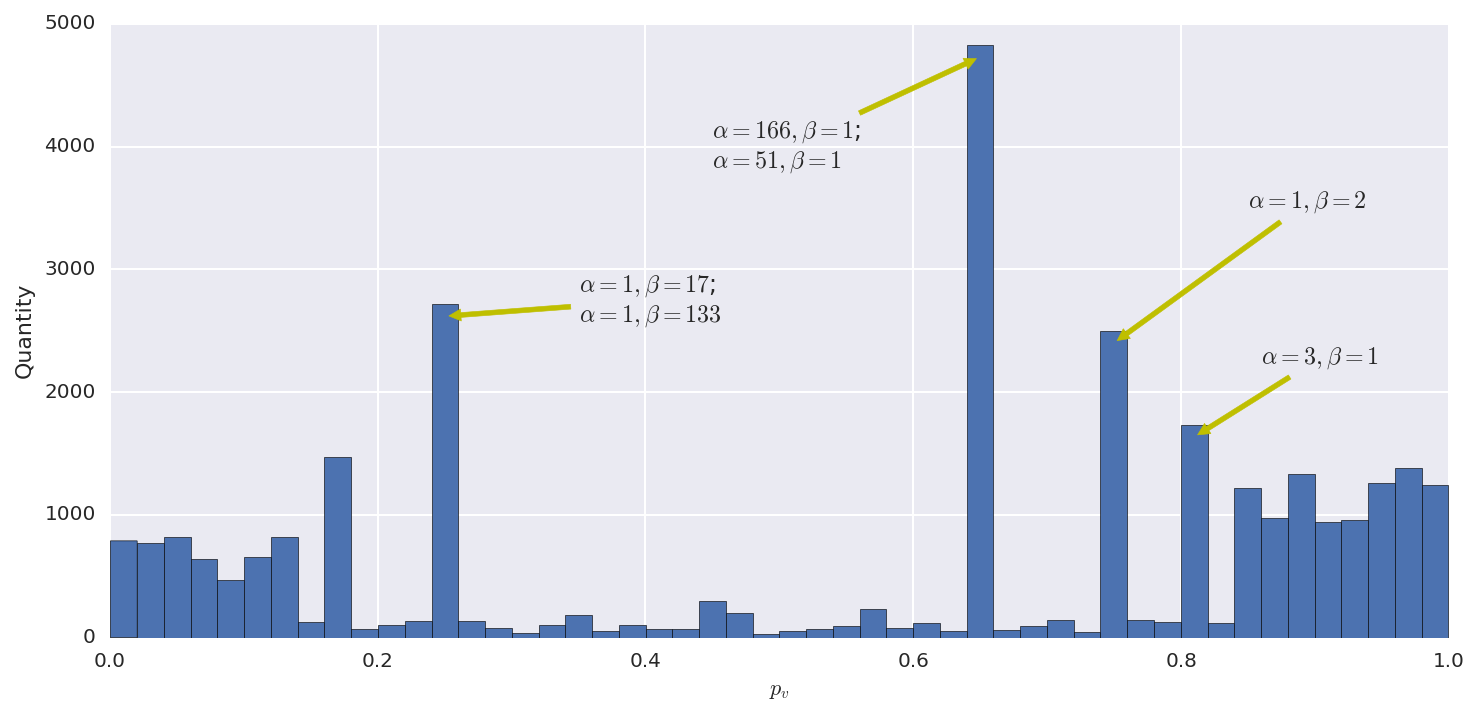
\includegraphics[width=\textwidth, height=.25\textheight, keepaspectratio]{figures/bayes/hist_calls.png}
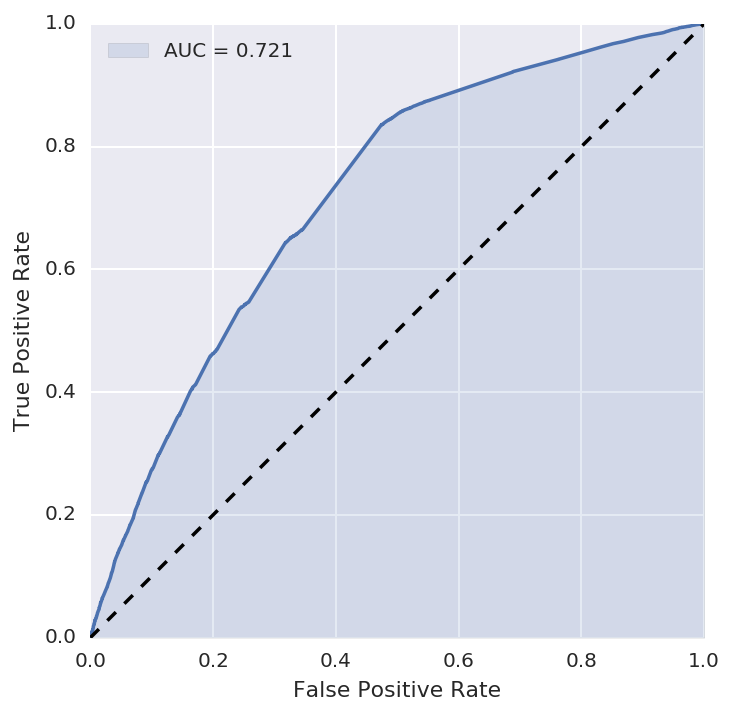
\includegraphics[width=.49\textwidth, height=.25\textheight, keepaspectratio]{figures/bayes/roc_calls.png}
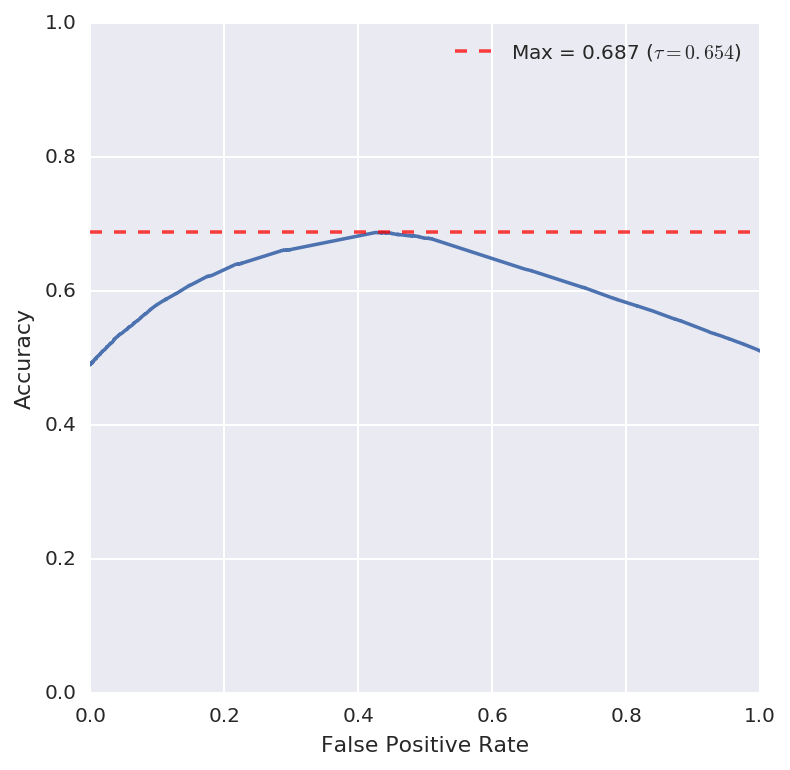
\includegraphics[width=.49\textwidth, height=.25\textheight, keepaspectratio]{figures/bayes/accuracy_calls.png}
\caption{Results of the \emph{Bayesian Algorithm} for call data.}
\label{fig:bayes_calls}
\end{figure}

\Cref{fig:bayes_calls} contains data about the predictor when $\varpi = \calls$ and the data is analyzed using $\Upsilon^{\calls}$ as \emph{Testing Set}. The \emph{Inverse Cumulative Distribution Function} contains a few peaks for users with a similar amount of calls.

After analyzing the data, we find that the \emph{Area Under the Curve} using this method is of \num{0.724}, which is significantly higher than all the naïve and \emph{Machine Learning} methods that will be presented in the later \cref{sec:comparison}.

Setting $\tau = 0.654$ maximizes the accuracy at $\Accuracy = 0.687$. Additionally, that value of $\tau$ results in $\Precision = 0.653$, $\Recall = 0.815$, $F_1 = 0.725$, and $F_4 = 0.804$.

\newpage

\subsection{Inferring by Time}
\label{subsec:time_infer}

\begin{figure}[h]
\centering
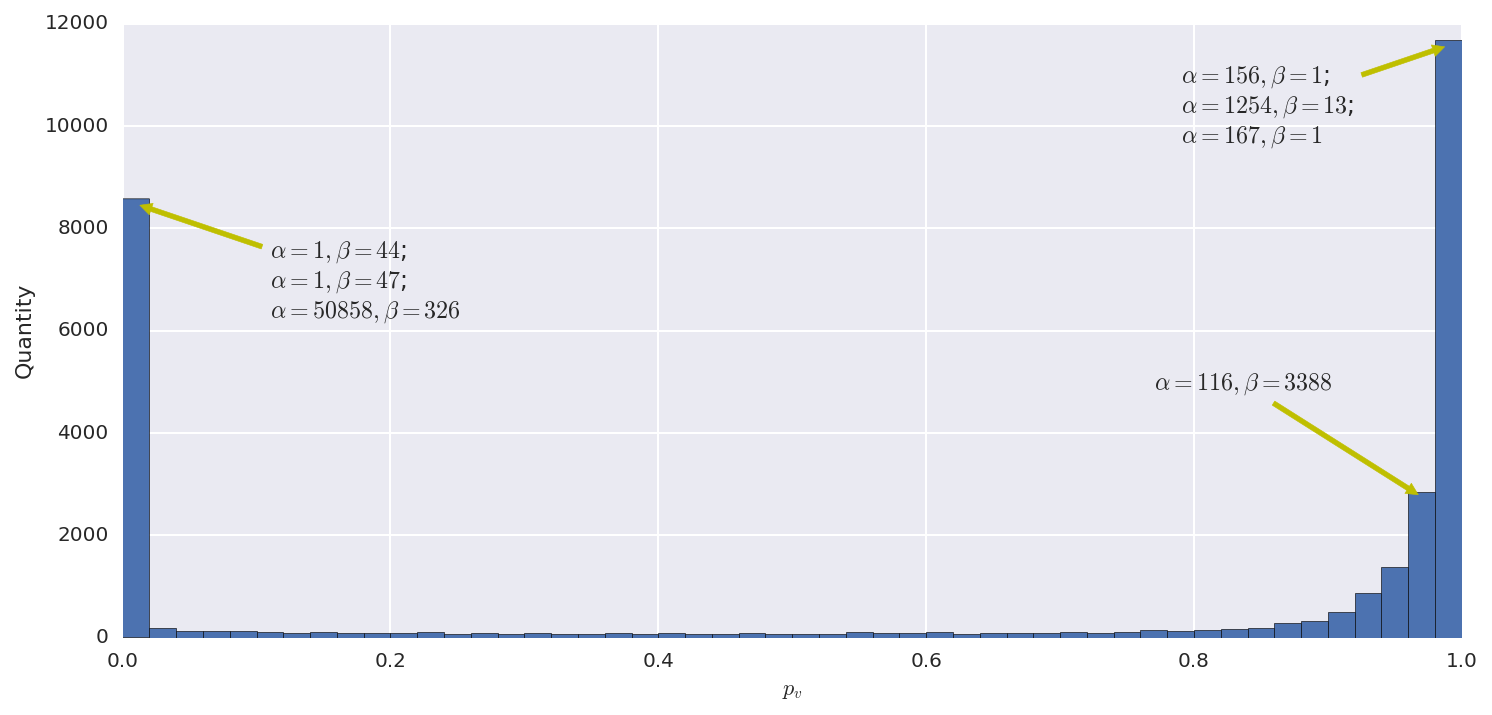
\includegraphics[width=\textwidth, height=.25\textheight, keepaspectratio]{figures/bayes/hist_time.png}
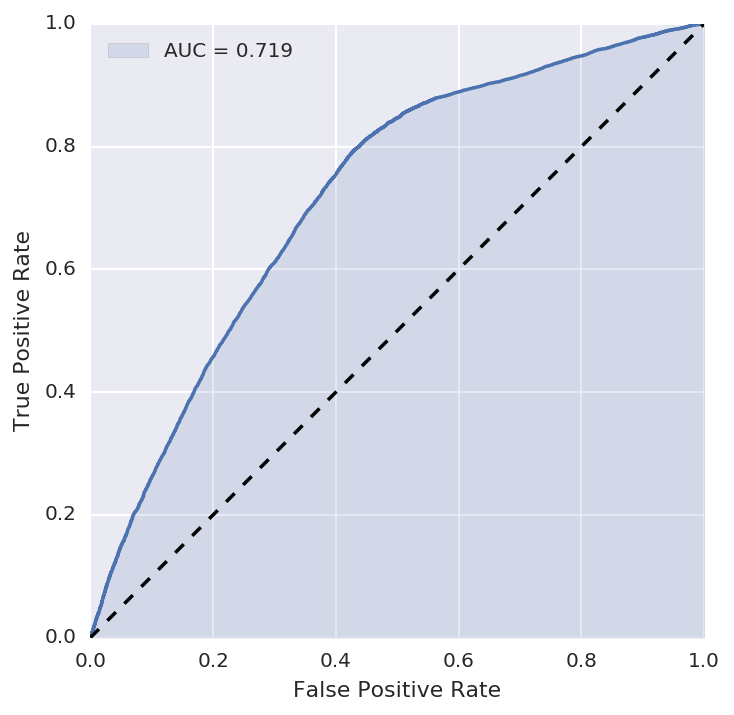
\includegraphics[width=.49\textwidth, height=.25\textheight, keepaspectratio]{figures/bayes/roc_time.png}
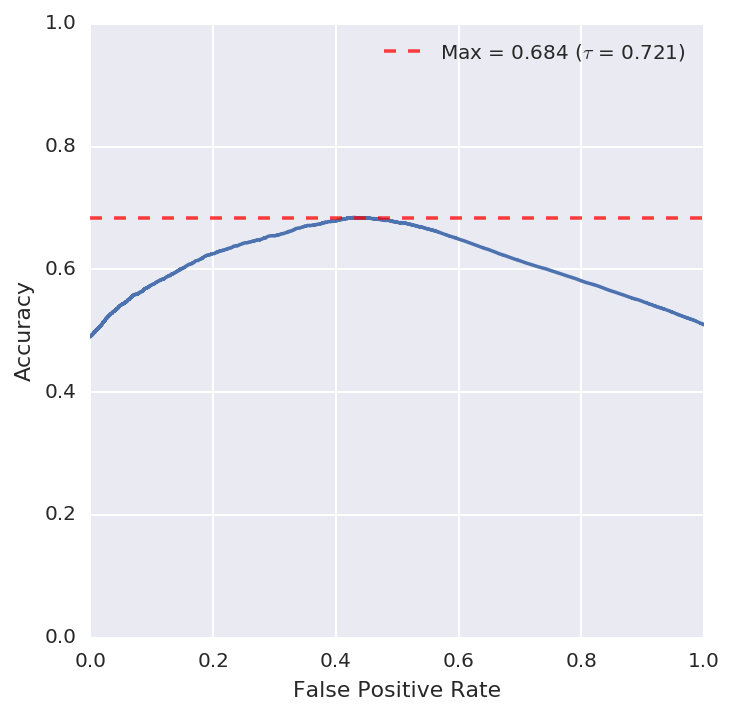
\includegraphics[width=.49\textwidth, height=.25\textheight, keepaspectratio]{figures/bayes/accuracy_time.png}
\caption{Results of the \emph{Bayesian Algorithm} for time data.}
\label{fig:bayes_time}
\end{figure}

\Cref{fig:bayes_time} contains data about the predictor when $\varpi = \etime$ and the data is analyzed using $\Upsilon^{\calls}$ as \emph{Testing Set}, there are two big clusters of data at the edges; this is explained because the majority of users spend most of their time talking to either \emph{High Income} or \emph{Low Income} users.

The \emph{Area Under the Curve} of this inference mechanism is $\AUC = 0.718$, which is lower than the one for the calls in \cref{subsec:calls_infer}. The \emph{Accuracy Curve} is unsurprisingly similar to that one, and even the \emph{Accuracy} at $\tau = 0.722$ is the close. This is probably a result of the fact that there is an obvious correlation between total talking time and total calls.

This $\tau$ also results in a predictor where $\Accuracy = 0.682$, $\Precision = 0.649$, $\Recall = 0.819$, $F_1 = 0.724$, and $F_4 = 0.807$.

\subsection{Inferring by SMS}
\label{subsec:sms_infer}

\begin{figure}[h]
\centering
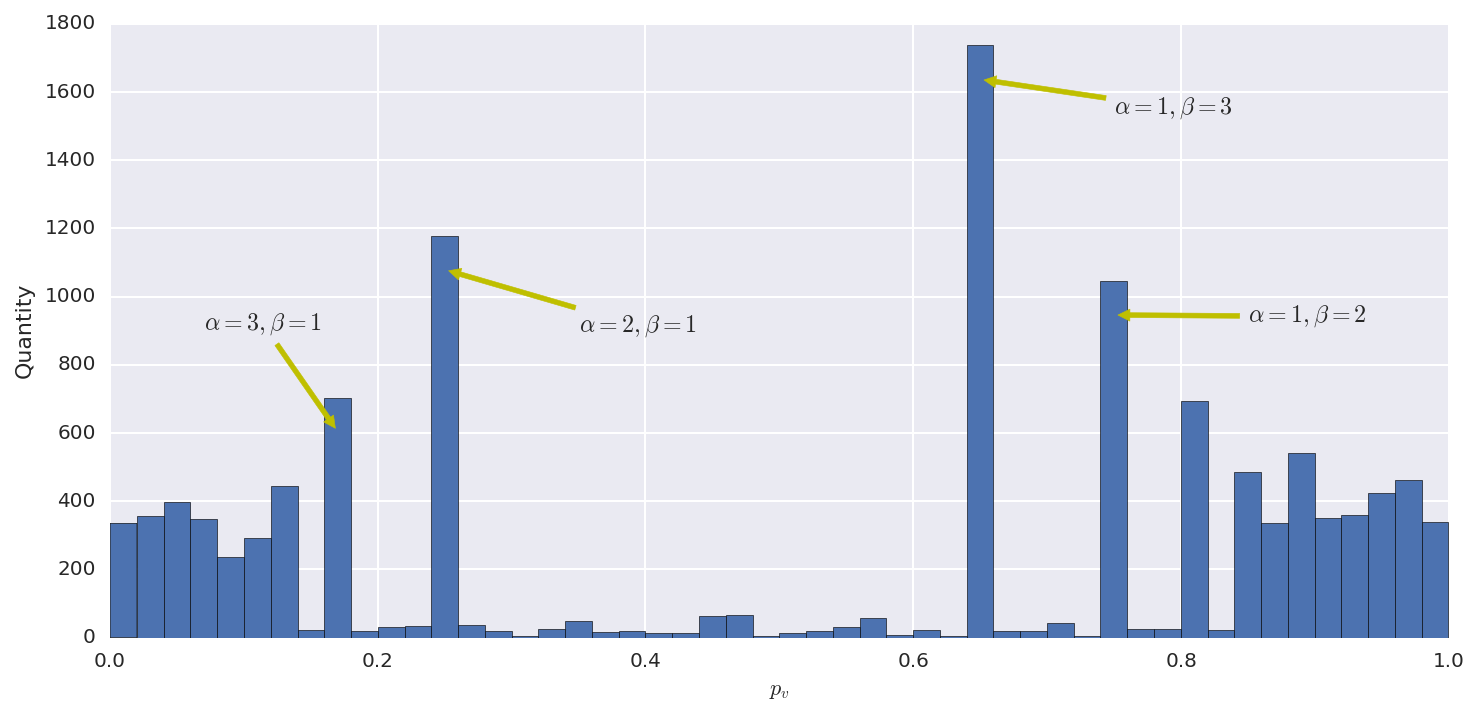
\includegraphics[width=\textwidth, height=.25\textheight, keepaspectratio]{figures/bayes/hist_sms.png}
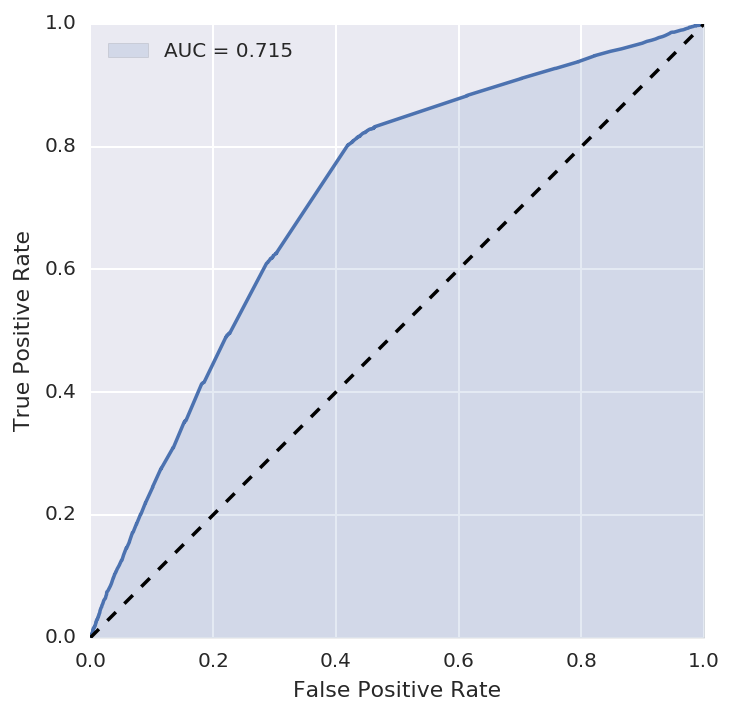
\includegraphics[width=.49\textwidth, height=.25\textheight, keepaspectratio]{figures/bayes/roc_sms.png}
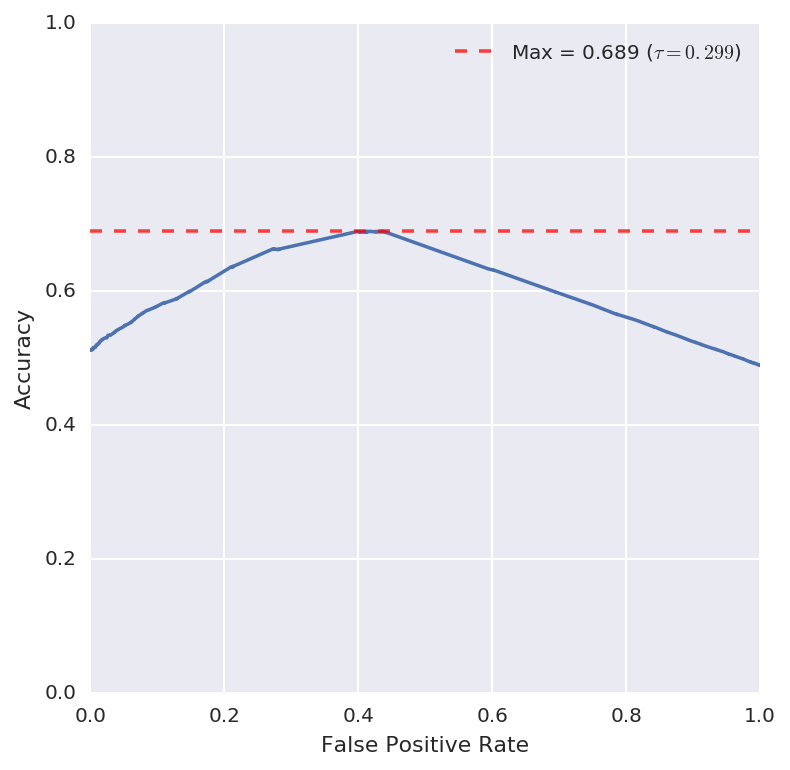
\includegraphics[width=.49\textwidth, height=.25\textheight, keepaspectratio]{figures/bayes/accuracy_sms.png}
\caption{Results of the \emph{Bayesian Algorithm} for SMS data.}
\label{fig:bayes_sms}
\end{figure}

\Cref{fig:bayes_sms} shows the distributions when $\varpi = \sms$. Since the total amount of SMS is much lower than the amount of calls, the peaks of the result of the \emph{Inverse Cumulative Functions} of the \emph{Beta Distribution} applied on $\Upsilon^{\sms}$ that happen with the majority of users that have few of both are located closer to the center than in \cref{subsec:calls_infer,subsec:time_infer}. This makes some interesting cases if $\varpi = \sms$ is chosen, since the distribution is different than in the other cases.

In particular, this gives an $\AUC = 0.715$, which is lower than both in the case of \emph{Calls} and \emph{Time}. Interestingly, the maximum \emph{Accuracy} at $\tau = 0.299$ is slightly higher than both of the other cases; this is probably a side-effect of the fact that $\left| \Upsilon^{\sms} \right| < \left| \Upsilon^{\calls} \right|$.

Additionally, $\Precision = 0.696$, $\Recall = 0.186$, $F_1 = 0.293$, and $F_4 = 0.194$.

\subsection{Inferring by Contacts}
\label{subsec:contacts_infer}

\begin{figure}[h]
\centering
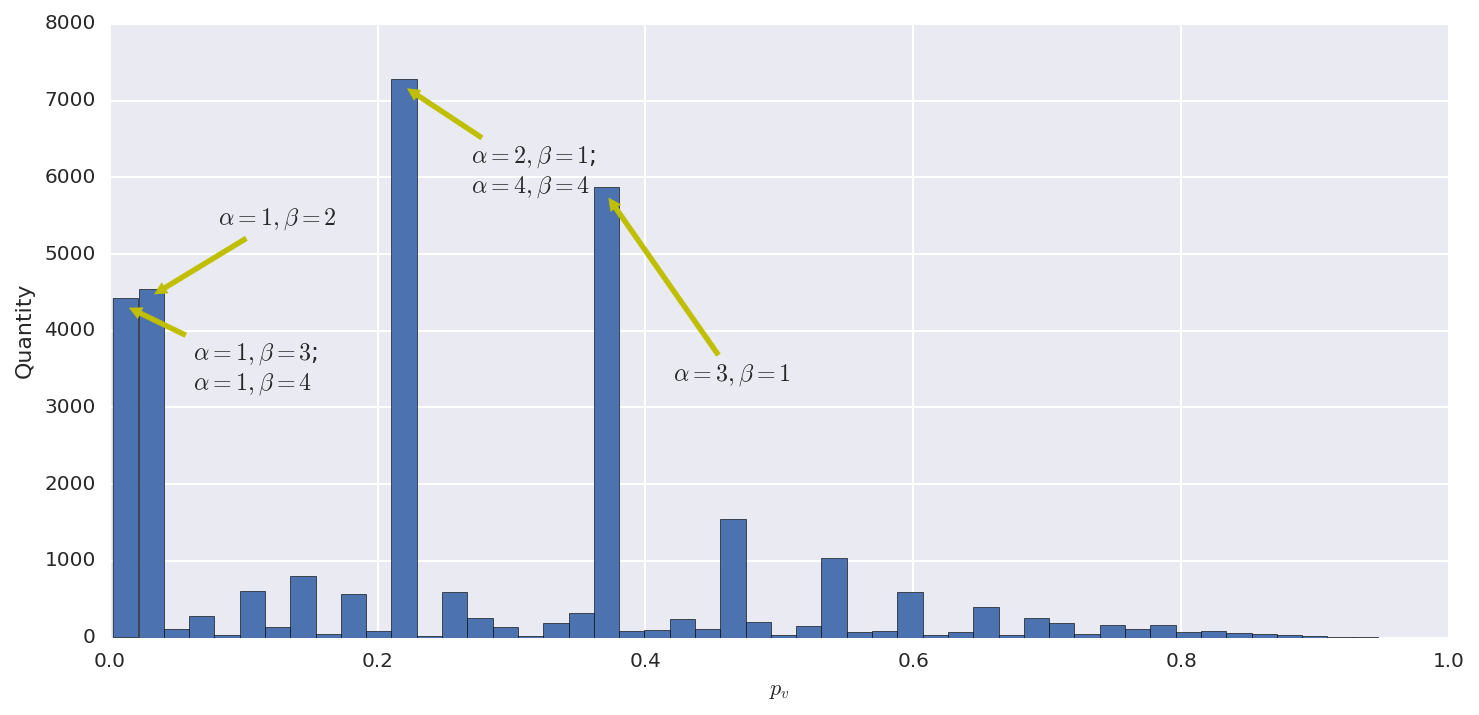
\includegraphics[width=\textwidth, height=.25\textheight, keepaspectratio]{figures/bayes/hist_contacts.png}
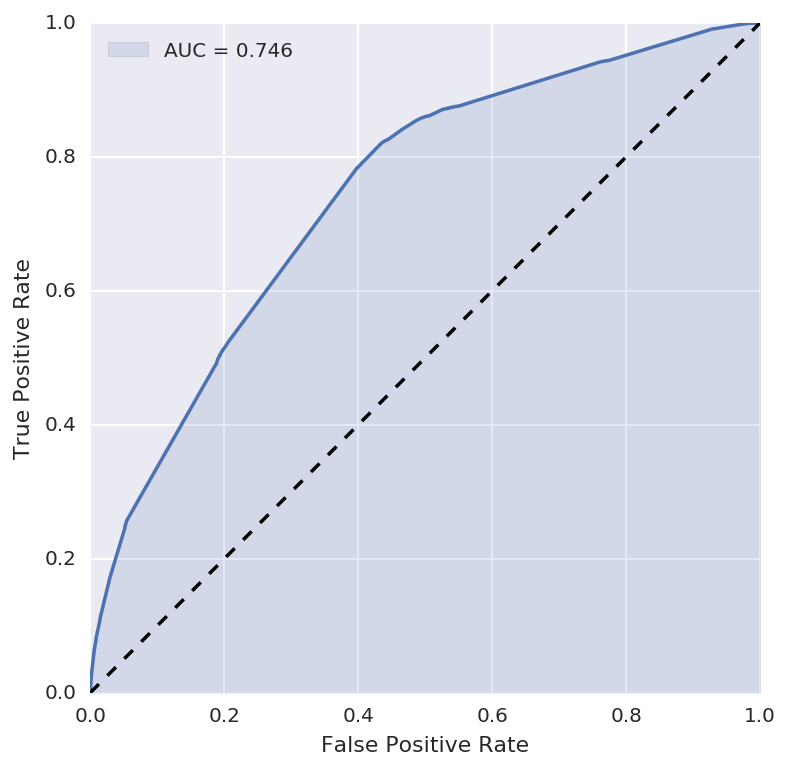
\includegraphics[width=.49\textwidth, height=.25\textheight, keepaspectratio]{figures/bayes/roc_contacts.png}
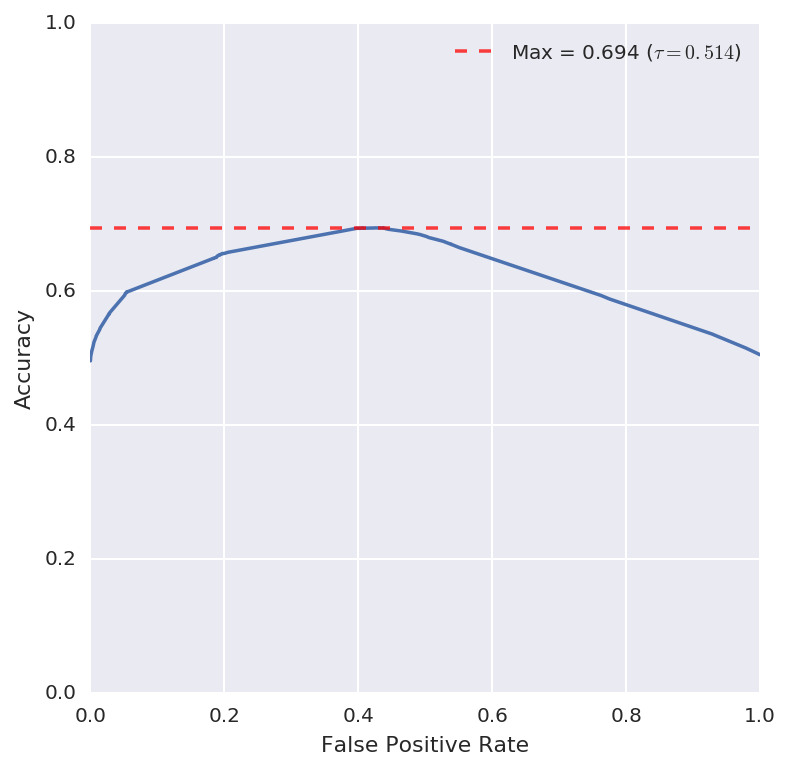
\includegraphics[width=.49\textwidth, height=.25\textheight, keepaspectratio]{figures/bayes/accuracy_contacts.png}
\caption{Results of the \emph{Bayesian Algorithm} for degree data.}
\label{fig:bayes_contacts}
\end{figure}

\Cref{fig:bayes_contacts} shows the distributions when $\varpi = \contacts$, where it is possible to get a pattern similar to the one shown in \cref{subsec:sms_infer} when $\varpi = \sms$, where the majority of users have relatively few contacts and the peaks in the histogram. Additionally, since the total amount of contacts is exponentially distributed (as shown in \cref{fig:outcontacts_dist}), and people with \emph{High Income} tend to have more contacts in general, there peaks are clustered in areas with low $p_v$ (where the majority of calls are made to \emph{Low Income} users), near the middle (where the calls are mostly equally distributed), but not at high $p_v$; this last section would belong to the few users with many calls to \emph{High Income} users.

Using this method it is possible to find that $\AUC = 0.746$, which is higher than all the other methods presented in \cref{subsec:algorithm_performance}. Additionally, when selecting $\tau = 0.514$, $\Accuracy = 0.694$ which is higher than the maximum \emph{Accuracy} in all other methods. These metrics, combined with the fact that $\Upsilon$ contains every user in the \emph{Testing Set}, result in the fact that $\varpi = \contacts$ is unambiguously the best way to classify the data for the algorithm. Additionally, $\Precision = 0.556$, $\Recall = 0.792$, $F_1 = 0.723$, and $F_4 = 0.783$.

\subsection{Final Results}

\Cref{tab:bayesresults} presents every metric discussed in \cref{subsec:mlmetrics} for the optimal $\Theta$ and $\tau$ for every $\varpi$.

\begin{table}
\centering
\begin{tabular}{>{\bfseries}l >{\hspace{1em}}r r >{\hspace{1em}}r r r r r r}
\toprule
$\varpi$ & \ct{$\Theta$} & \ct{$\tau$} & \ct{Acc.} & \ct{Prec.} & \ct{Rec.} & \ct{AUC} & \ct{F\textsubscript{1}} & \ct{F\textsubscript{4}} \\
\midrule
calls    & 0.428 & 0.654 & 0.686 & 0.654 & 0.816 & 0.724 & 0.726 & 0.804 \\
time     & 0.001 & 0.722 & 0.681 & 0.652 & 0.806 & 0.718 & 0.721 & 0.795 \\
sms      & 0.428 & 0.299 & 0.688 & 0.648 & 0.789 & 0.715 & 0.712 & 0.779 \\
contacts & 0.394 & 0.514 & 0.693 & 0.665 & 0.792 & 0.746 & 0.723 & 0.783 \\
\bottomrule
\end{tabular}
\caption{Metrics for the Bayesian algorithm using every user in $\Upsilon$}
\label{tab:bayesresults}
\end{table}

In particular, the results show that using \emph{Contacts} as the predictor for the \emph{Bayesian Algorithm} results in a significantly higher \emph{Area Under the Curve} and a higher \emph{Accuracy}.

\section{Algorithm Performance of Users with at least 3 Contacts}

The algorithm tends to be a better predictor of the \emph{Socioeconomic Level} for users with high amount of information on the graph $G$, namely that the amount of users in their neighborhood that also belong to $B$ is big.

In this section, we run the \emph{Bayesian Algorithm} for the subset of the users presented in \cref{eq:3contacts}, which restrict the users in the \emph{Testing Set} to only those who have at least 3 contacts. This would allow us to have better metrics in the dataset, at the expense of a much smaller Universe of users for which the algorithm could be applied. Additionally, \cref{tab:3contacts} shows the sizes of the \emph{Testing Sets} used in a manner similar to \cref{tab:partition_numbers}.

\begin{equation}
\label{eq:3contacts}
\begin{gathered}
I = \left\{ \upsilon \in \Upsilon \mid \contacts^{high}_{\upsilon} + \contacts^{\low}_{\upsilon} > 3 \right\} \\
I^{\calls} = \Upsilon^{\calls} \cap I
\end{gathered}
\end{equation}

\begin{table}
\centering
\begin{tabular}{l r r r c}
\toprule
Set & Total Size & High Income & Low Income & Ratio \\
\midrule
$I$ & \num{7932} & \num{4637} & \num{3295} & \num{0.258} \\
$I^{\calls}$ & \num{7910} & \num{4627} & \num{3283} & \num{0.214} \\
\bottomrule
\end{tabular}
\caption{Amount of users in the \emph{Testing Set} after trimming it several to only have users with at least 3 contacts.}
\label{tab:3contacts}
\end{table}

\subsection{Inferring by Calls on Users with at least 3 Contacts}

\begin{figure}[tbh]
\centering
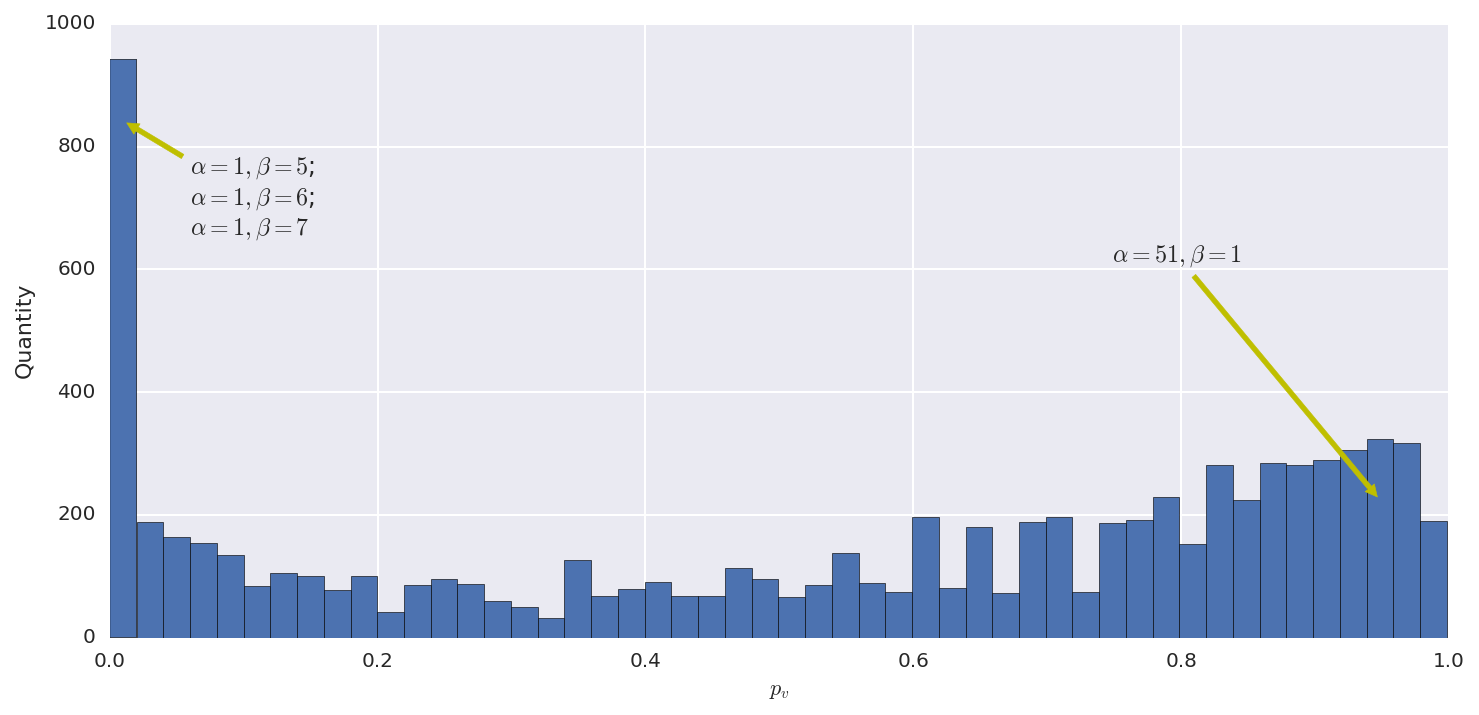
\includegraphics[width=\textwidth, height=.25\textheight, keepaspectratio]{figures/bayes/3contacts/hist_calls.png}
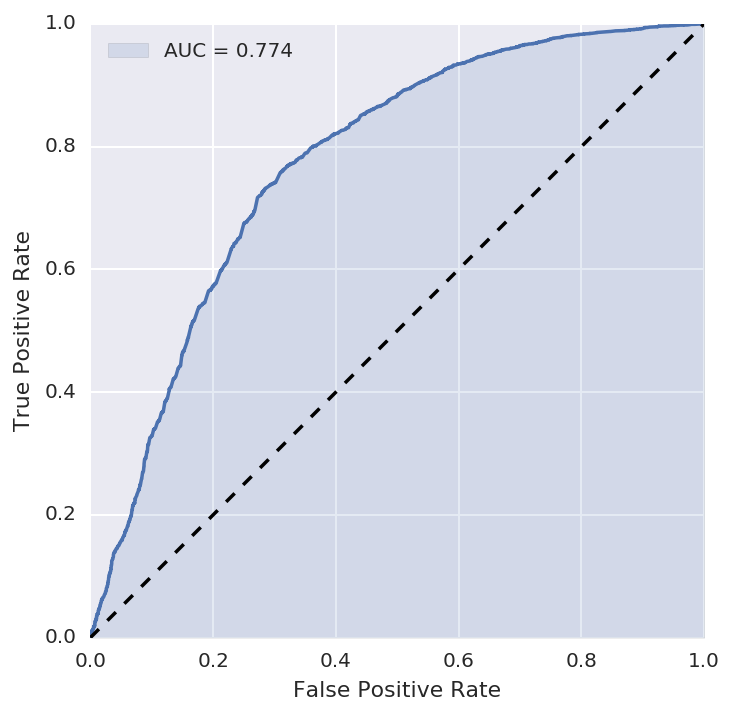
\includegraphics[width=.49\textwidth, height=.25\textheight, keepaspectratio]{figures/bayes/3contacts/roc_calls.png}
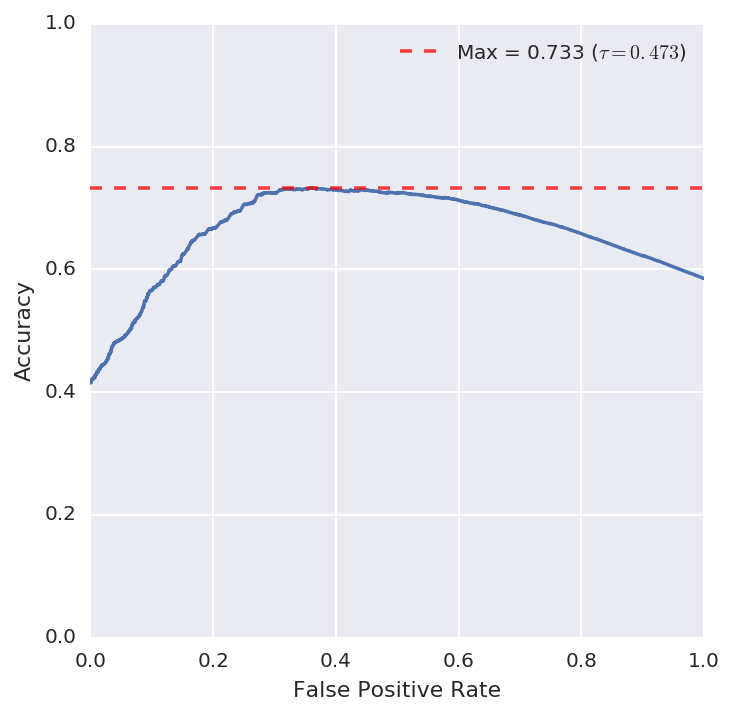
\includegraphics[width=.49\textwidth, height=.25\textheight, keepaspectratio]{figures/bayes/3contacts/accuracy_calls.png}
\caption{Results of the \emph{Bayesian Algorithm} for call data by only counting users with at least 3 contacts.}
\label{fig:bayes_calls_least3}
\end{figure}

\Cref{fig:bayes_calls_least3} uses $I^{\calls} \subseteq \Upsilon^{\calls}$ and $\varpi = \calls$ to create a predictor where both the \emph{Area Under the Curve} and the \emph{Accuracy} are higher than in all predictors that use every possible user. However, this data predicts less users and is strictly worse than the one presented in the following section.

\subsection{Inferring by Degree on Users with at least 3 Contacts}

\begin{figure}[tbh]
\centering
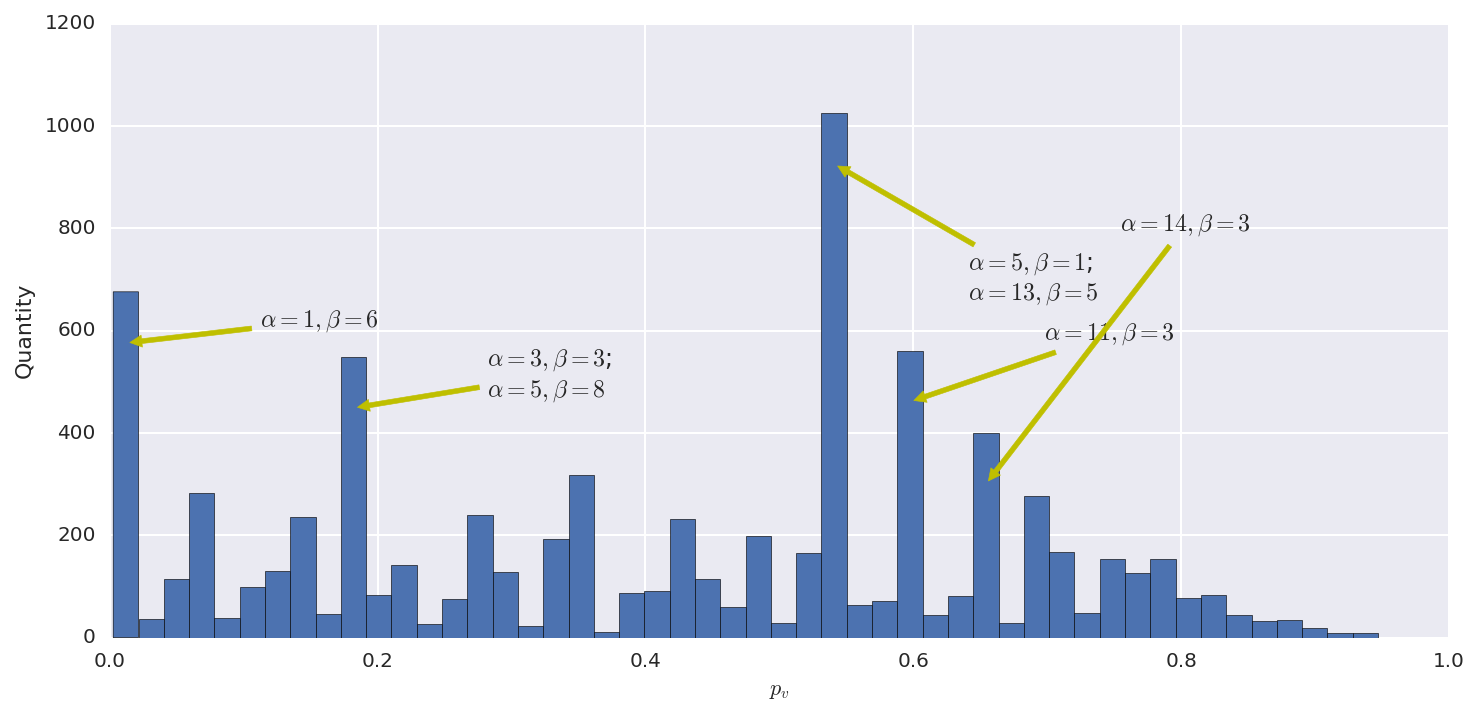
\includegraphics[width=\textwidth, height=.25\textheight, keepaspectratio]{figures/bayes/3contacts/hist_contacts.png}
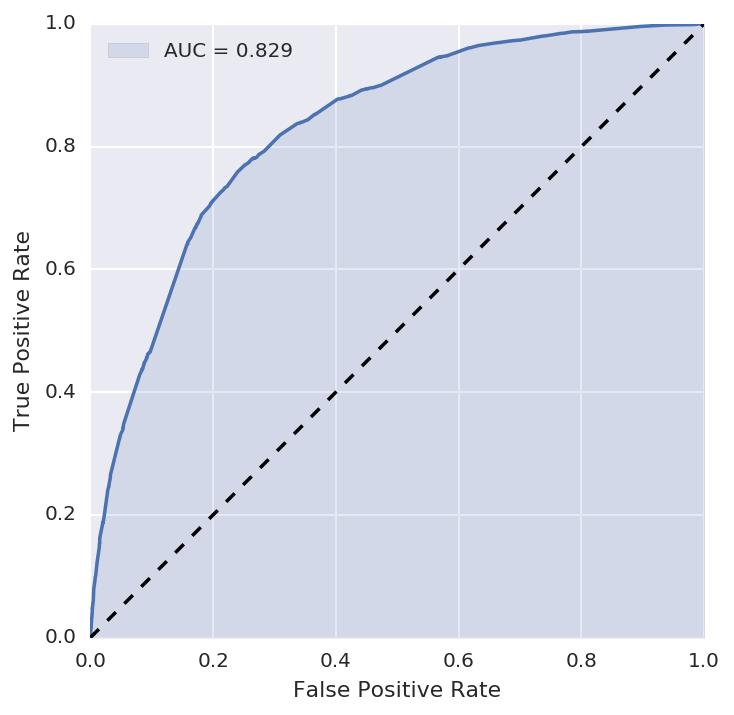
\includegraphics[width=.49\textwidth, height=.25\textheight, keepaspectratio]{figures/bayes/3contacts/roc_contacts.png}
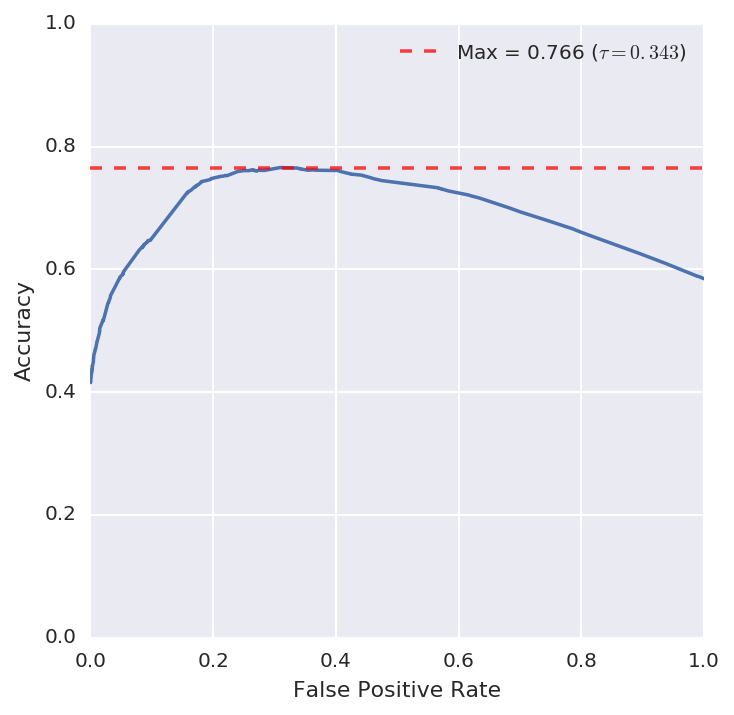
\includegraphics[width=.49\textwidth, height=.25\textheight, keepaspectratio]{figures/bayes/3contacts/accuracy_contacts.png}
\caption{Results of the \emph{Bayesian Algorithm} for contacts data by only counting users with at least 3 contacts.}
\label{fig:bayes_contacts_least3}
\end{figure}

The results in \cref{fig:bayes_contacts_least3} show the best possible predictor for a reasonable subset of the users. Both the \emph{Area Under the Curve} and the \emph{Accuracy} are higher than for all other predictors, with $\AUC = 0.829$ and $\Accuracy = 0.766$.

All of those values are considerably better than any other predictor in this page at the cost of using only a small subset of the possible users. This is interesting as it is exactly the same subset as the one used in~\cite{fixman2016bayesian}, and it scores significantly higher in all the metrics.
